\documentclass[10pt]{article}
\newcommand{\HRule}{\rule{\linewidth}{0.5mm}}
\parindent 0pt
\parskip 10pt
\usepackage{anysize}
\usepackage{graphicx}
\usepackage{epsfig}
\usepackage{float}
%\usepackage{cite}
\usepackage{natbib}
\usepackage{setspace}
\marginsize{3.5cm}{3.5cm}{1cm}{1cm}
\onehalfspacing
\usepackage{caption}
\usepackage{subcaption}
\usepackage{amsmath}

%\textwidth 15cm
%\textheight 24cm
%\onehalfspacing
\begin{document}

\title{Tennis Challenge Solution}

\author{David Starkey}

\maketitle


\section{Statistics of Tennis}
In the following short study, I investigate the probability of various outcomes of a set of tennis. The set is won when either of two players have reached 6 games AND are ahead by two clear games. A game is won when a player wins four rallies AND are ahead by two clear points. The investigation will examine how the probability of winning a set of tennis (the set-win probability) is affected by a players point-win probability (the probability of the player winning a single rally). The statistical framework for the study is described in the following sections and the accompanying code will allow the interested reader to duplicate the figures and analysis below for any desired point-win probability. I aim to:

\begin{itemize}
\item Examine landscape of the 2D posterior probability distribution as a function of all possible scores.

\item Examine how the set-win probability evolves with point-win probability (in other words how much more likely are you to win a set given a particular probability of scoring a rally). 

\end{itemize}

I hope you have fun!

\section{Probabilty of Winning Game}
This is the sum of two possible outcomes.

\begin{equation}
\label{eq_pwg}
P(wg) = P( \mathrm{wbd} ) + P( \mathrm{g2d} ) \times P(\mathrm{wod})
\end{equation}
\noindent where the probabilities of winning before deuce, of the game reaching deuce, and of winning a deuce are given by $P( \mathrm{wbd} )$, $P( \mathrm{g2d} )$ and $P(\mathrm{wod})$ respectively.



\subsection{Probability of Reaching Deuce: P(g2d)}

A game will reach deuce if C(W W W L L L), where C denotes the events can happen in any order, and yet the same event is described by reversing the positions of two W's. We therefore need to avoid double counting of events using the factorials below. This has the probability given by
\begin{equation}
\label{eq_g2d}
P(\mathrm{g2d}) = \frac{6!}{3!3!}p^3 ( 1 - p)^3.
\end{equation}


\subsection{Probability of Winning Before Deuce: $P ( \mathrm{wbd} )$ }
This will occur in any of the following circumstances.
\begin{equation}
\label{eq_C}
\begin{split}
C(\mathrm{W W W W}) = p^4, \\
C(\mathrm{W W W L}) \mathrm{W} = \frac{4!}{3!1!}p^3 (1-p) p, \\
C(\mathrm{W W W L L}) \mathrm{W} = \frac{5!}{3!2!}p^3 (1-p)^2 p. \\
\end{split}
\end{equation}
\noindent The probability of winning before deuce is then the sum of these

\begin{equation}
\label{eq_pwbd}
P(\mathrm{wbd}) = p^4 \left( 1 + \frac{4!}{3!1!} (1-p) + \frac{5!}{3!2!}(1-p)^2 \right).
\end{equation}



\subsection{Probability of Winning Deuce: $P(\mathrm{wod})$}
To proceed further we need the probability of returning to deuce $P(\mathrm{b2d})$.
\begin{equation}
\label{eq_pb2d}
P(\mathrm{b2d}) = C(WL) = 2p(1-p)
\end{equation}

\noindent The game can now potentially last forever, continuously returning to deuce with diminishing probability. The probability of winning after $n$ deuces is. 
\begin{equation}
P(\mathrm{wnd}) = P(\mathrm{b2d})^{n-1} p^2.
\end{equation}

Since we can win on any of the $n$ deuces up to infinity we must evaluate the sum
\begin{equation}
\label{eq_wodpre}
P(\mathrm{wod}) = \sum_{n=1}^\infty P(\mathrm{b2d})^{n-1} p^2.
\end{equation}

\noindent For a geometric series of the form $a r^{n-1}$, the sum to infinity is $a_1 / (1 - r)$, with first term and common ratio $a_1$ and $r$. Combining this with Equation \ref{eq_wodpre}, we get the probability of winning a deuce (or of winning game by two clear points),

\begin{equation}
\label{eq_wod}
P(\mathrm{wod}) = \frac{p^2}{1 - 2p(1-p)}.
\end{equation}

\noindent Combining Equations \ref{eq_pwg}, \ref{eq_wod} and \ref{eq_g2d} gives us the explicit probability of winning a game.

\begin{equation}
\label{eq_pwgexp}
P(\mathrm{wg}) = p^4 \left( 1 + \frac{4!}{3!1!} (1-p) + \frac{5!}{3!2!}(1-p)^2 \right) + \frac{6!}{3!3!}p^3 ( 1 - p)^3 \frac{p^2}{1 - 2p(1-p)}.
\end{equation}

\noindent This gives us the probability of winning a game. We now do a similar procedure, taking $P(\mathrm{wg})$ forward to calculate the set win probability.



\section{Probability of Winning Set: $P_s(X,X)$}
To win a set, we need to get to 6 points and be in the lead by 2 clear points. If both players reach 6, a tie break game determines the final set and winner. Using the same reasoning as Equation \ref{eq_C} I calculate the possible winning scores and probabilities as

\begin{equation}
\label{eq_swin}
\begin{split}
P_s(6,0) = C(\mathrm{WWWWWW}) = p_g^6, \\
P_s(6,1) = C(\mathrm{WWWWWL}) W = \frac{6!}{5!1!}p_g^5 (1-p_g) p_g, \\
P_s(6,2) = C(\mathrm{WWWWWLL}) W = \frac{7!}{5!2!}p_g^5 (1-p_g)^2 p_g, \\
P_s(6,3) = C(\mathrm{WWWWWLLL}) W = \frac{8!}{5!3!}p_g^5 (1-p_g)^3 p_g, \\
P_s(6,4) = C(\mathrm{WWWWWLLLL}) W = \frac{9!}{5!4!}p_g^5 (1-p_g)^4 p_g, \\
P_s(7,5) = C(\mathrm{WWWWWLLLLL}) WW = \frac{10!}{5!5!}p_g^5 (1-p_g)^5 p_g^2, \\
P_s(7,6) = P(\mathrm{g266}) p_g,
\end{split}
\end{equation}
\noindent where the point probability $p$ has been replaced by the probability of winning a game $p_g = P(\mathrm{wg})$ (see Equation \ref{eq_pwg}). These are calculated by suitably combining probabilities and noting that the some ordering of W and L are the same event. I try to encapsulate this meaning in the C() functions. The interesting case is that of the tie break $P_s(7,6)$. To win a tie break, we first have to reach a score of 5,5. This is given by $P(\mathrm{g255})$ where

\begin{equation}
\label{eq_p55}
P(\mathrm{g255}) = C(\mathrm{WWWWWLLLLL}) = \frac{10!}{5!5!}p_g^5 (1-p_g)^5.
\end{equation}
\noindent The probability of reaching a score of 6,6 is then
\begin{equation}
\label{eq_p66}
P(\mathrm{g266}) = P(\mathrm{g255})p_g (1-p_g) + P(\mathrm{g255} (1-p_g)p_g = 2P(\mathrm{g255}p_g (1-p_g),
\end{equation}
\noindent since we can first win and then lose or vice versa. Combining Equations \ref{eq_p66} and \ref{eq_swin} gives us the full range of probabilities for an input point probability $p$ and score. To consider losing the set, I simply replace $p_g$ with $1-p_g$ in Equation \ref{eq_swin} and consider a win $W$ now to be a loss $L$.






\section{Posterior Probability Landscape}
The statistical analysis below can be coded into a Python script without too much hassle and allows us to investigate the probability of various game scores for the set. Figure \ref{fig_posterior} shows this landscape for a game between Player 1 and Player 2 when Player 1 has a point-win probability of 0.45 (and Player 2 has a point-win probability of 0.55), 0.50 and 0.55 respectively. 


\begin{figure*}
\centering
	\begin{tabular}{@{}ccc@{}}
	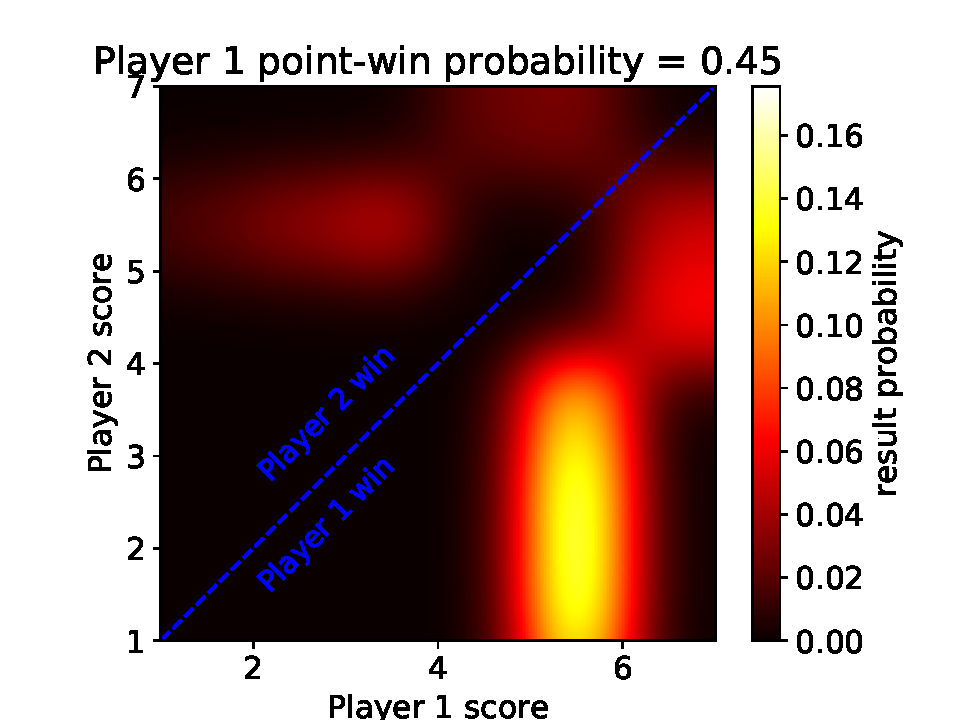
\includegraphics[width=0.72\textwidth]{tenplot_point4.pdf}\\
	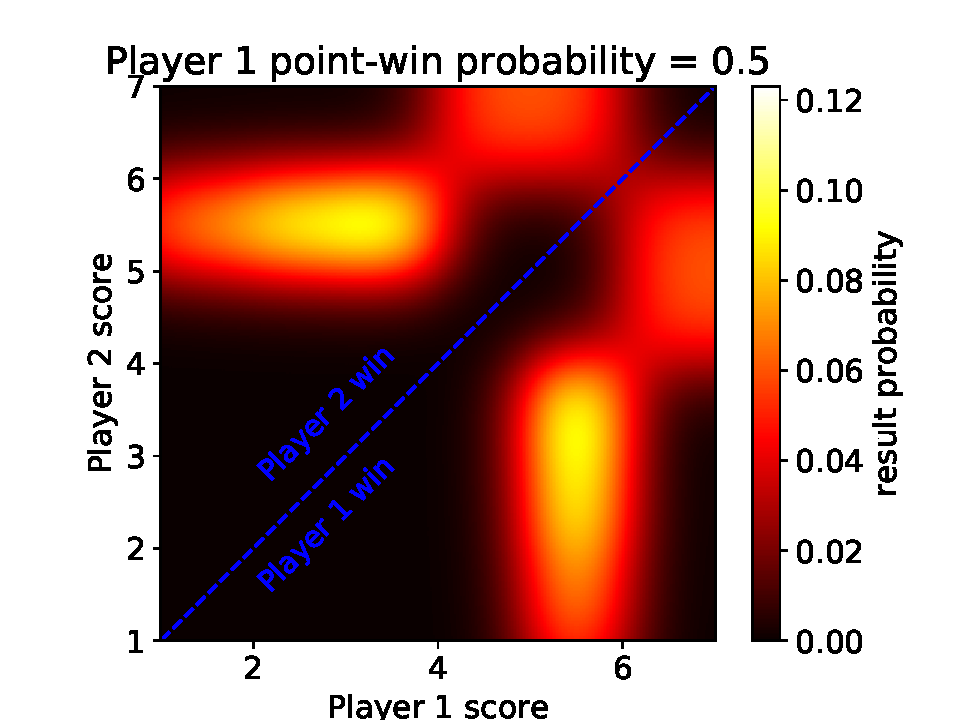
\includegraphics[width=0.72\textwidth]{tenplot_point5.pdf}\\
	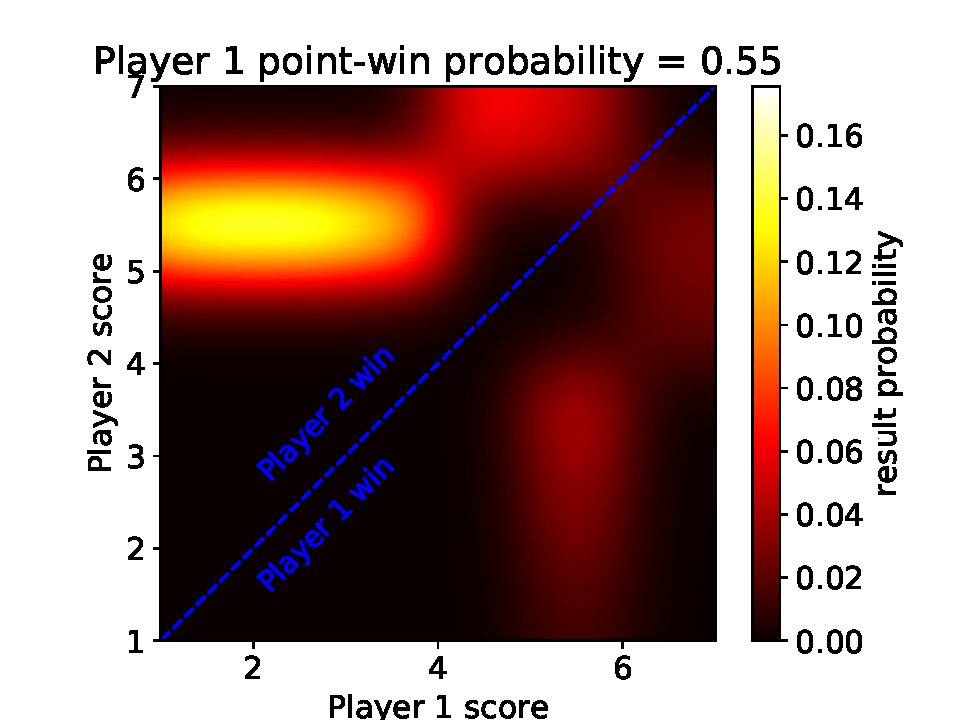
\includegraphics[width=0.72\textwidth]{tenplot_point6.pdf}
	\end{tabular}
    \caption{The 2-D posterior probability landscape as a function of the various scores. Black points indicate invalid scores where the blue line divides a Player 1 victory from a Player 2 victory. The image headers show the input point-win probability for Player 1.}
    \label{fig_posterior}
\end{figure*}




\begin{figure}
\centering
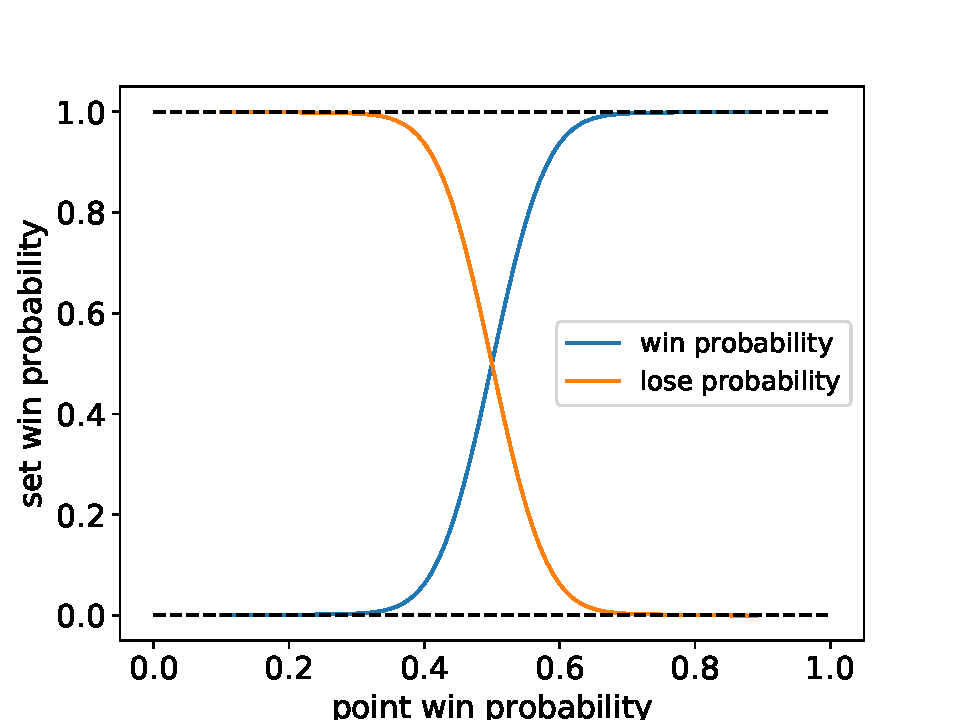
\includegraphics[width=0.92\textwidth]{fig_prob_point_set.pdf}
    \caption{The set-win probability vs the point-win probability. Dashed lines indicate the lower and upper limits zero and one. }
    \label{fig_point_set_win}
\end{figure}


\section{Conclusion}

A number of interesting features can be concluded from the posterior probability data in Figures \ref{fig_posterior} and \ref{fig_point_set_win}:

\begin{itemize}

\item Figure \ref{fig_posterior} shows that the posterior probability landscape is very sensitive to the point-win probability; a slight imbalance of the point-win probability is all that is needed to make a Player significantly more likely to win the set.

\item The above point is illustrated more dramatically in Figure \ref{fig_point_set_win}. This shows the probability of winning a set given the probability of winning a point. This is not linear (a 10 \% increase in the probability of winning a rally does not correspond to the same increase in winning a set). The steep increase of the curve around 0.4 shows how quickly a point-win advantage conveys a much higher set-win probability.

\end{itemize}


Future considerations in this study might build on the set-win probability study and investigate the match-win probability. This is a very simple rule addition to the code where match is the best of three (or five) sets and to win by two clear sets. One could also adapt the rules to other similar court games such as squash. The statistics of games is a very interesting field of study.





\end{document}



